\documentclass[a4paper]{article}

\usepackage[utf8]{inputenc}
\usepackage{fullpage} % Package to use full page
\usepackage{parskip} % Package to tweak paragraph skipping
\usepackage{amsmath}
\usepackage{hyperref}
\usepackage{graphicx}
\usepackage[croatian]{babel}

% TODO: align, verbatim, equation blocks

\renewcommand{\figurename}{Slika}

\title{Rangirajući pretraživač dokumenata - Infinity}
\author{Marko Budiselić}
\date{30.11.2015.}

\begin{document}

\maketitle

\section{Predprocesiranje}

\section{Algoritmi}

\subsection{Bag of words}

\subsection{Vector space}

\subsection{Binary independence}

\section{Upute za pokretanje}

\url{https://infinity.buda.link}

TODO: source setup.py

\section{Produkcijska okolina}

Svi upiti klijenata dolaze na Nginx load balancer koji ima izrazito veliku propusnost. Nakon toga load banancer prosljedjuje upit na worker instance koje svaka za sebe imaju cijeli dataset i znaju vratiti odgovarajuci rezultat. Dataset worker instance preuzimaju od db interface instance, a ne direktno iz baze. Trenutno je u deploymentu samo jedna instanca sucelja prema bazi, ali u produkciji tu moze biti opet load balancer i vise instanci interface-a prema bazi podataka. Baza podataka je MongoDB, takodjer samo jedna instanca, no u praksi tu moze doci mongo replica set ili mongo shard cluster.

Kao sto se vidi na grafu \ref{production_environment}, sve instance imaju simbolicka imena (FQDN). To je takodjer izrazito bitno jer se time postize transparentnost pristupa i migracijska transparentnost. U konkretnoj implementaciji sva imena su definirana u /etc/hosts file-u na deploy stroju, no u produkciji ce imene biti definirana na redundantnim DNS serverima.

\begin{figure}[!htbp]
\begin{center}
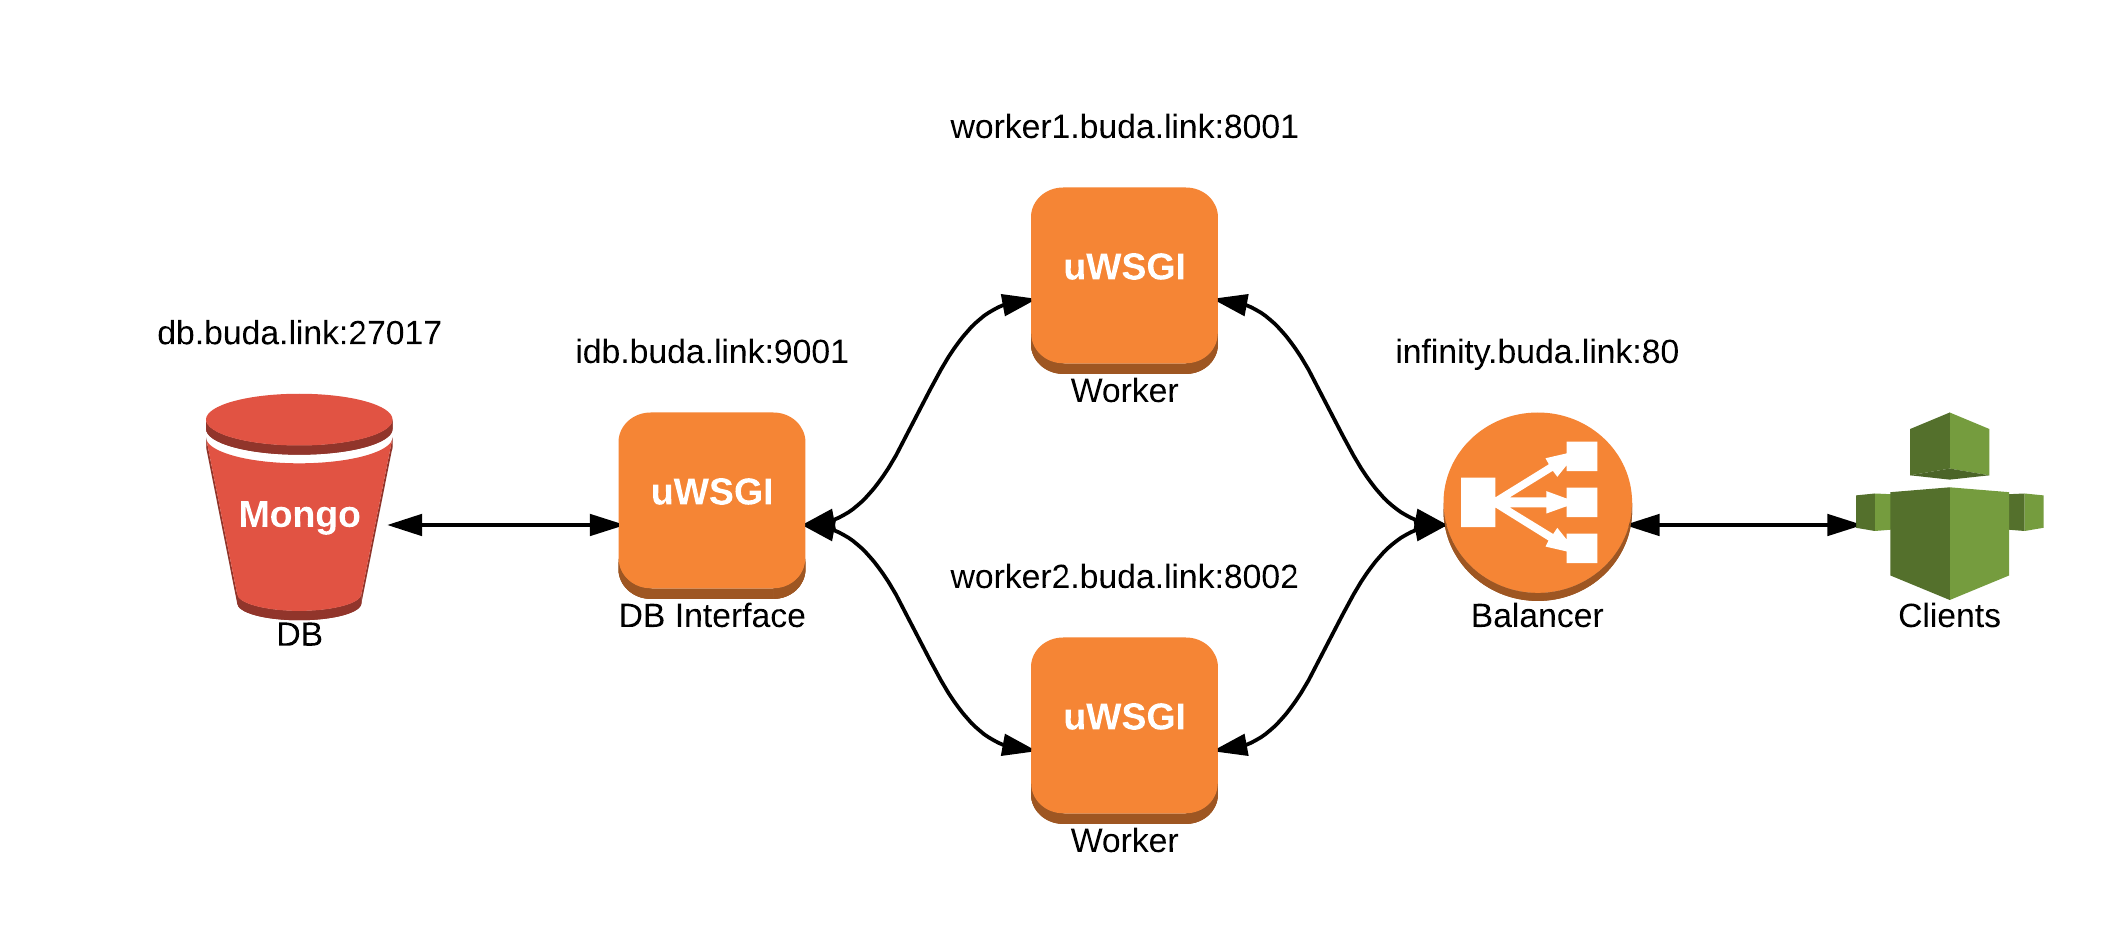
\includegraphics[width=\textwidth]{infinity.png}
\end{center}
\caption{Produkcijska okolina}\label{production_environment}
\end{figure}

\vspace{1cm}
P.S.
\\[0.3cm]
infinity $>$ gugol

\bibliographystyle{plain}
\bibliography{bibliography.bib}
\end{document}